\chapter{Setup}

% dark box
% power supplies
% multimeter
% osci
% gandalf + clock
% led + diffusor
% emusic
% sipm
\section{SiPM stuff}
The \acp{sipm} mainly used in this work are the \textit{S14160-3050HS} by the manufacturer Hamamatsu.
Another \ac{sipm} model used is the SensL \textit{J-Series 30035} manufactured by Onsemi.
Some important parameters of both \ac{sipm} models are listed in \autoref{tab:sipm_specs}.
For this work, \acp{pcb} with each forty \acp{sipm} of a model soldered onto it were used.
A picture of one of these \acp{pcb} equiped with Hamamatsu \acp{sipm} is shown in \autoref{fig:sipm_pcb}.

\begin{table}
	\centering
	\caption[SiPM parameters]{Relevant parameters of the both used \ac{sipm} models by Hamamatsu and Onsemi. \cite{}}
	\label{tab:sipm_specs}
	\renewcommand{\arraystretch}{1.3}
	\begin{tabularx}{\textwidth}{Xp{0.19\textwidth}p{0.15\textwidth}}
	    \toprule
	    parameter								& S14160-3050HS		& SensL			\\\midrule
	    photosensitive are / $\si{\milli\meter\squared}$			& 3.0$\times$3.0	& 3.07$\times$3.07	\\
	    pixel pitch / $\si{\micro\meter}$					& 50			& 35			\\
	    number of pixels							& 3000			& $\num{5676}$		\\
	    spectral response range / $\si{\nano\meter}$			& \numrange{270}{900}	& $\numrange{200}{900}$	\\
	    peak sensitivity wavenlength / $\si{\nano\meter}$			& 450			& 420			\\
	    peak photon detection eficiency / $\si{\percent}$			& 50			& 			\\
	    breakdown voltage / $\si{\volt}$					& 38			& \numrange{24.2}{24.7}	\\
	    recommended operating voltage / $\si{\volt}$			& 40.7			& \numrange{25.2}{30.7}	\\
	    variation of rec. op. voltage (typ. / max) / $\si{\volt}$		& 0.1 / 0.2		&			\\
	    gain								& \num{2.5e6}		&			\\
	    \bottomrule
	\end{tabularx}
	\renewcommand{\arraystretch}{1}
\end{table} 
\begin{figure}
	\centering
	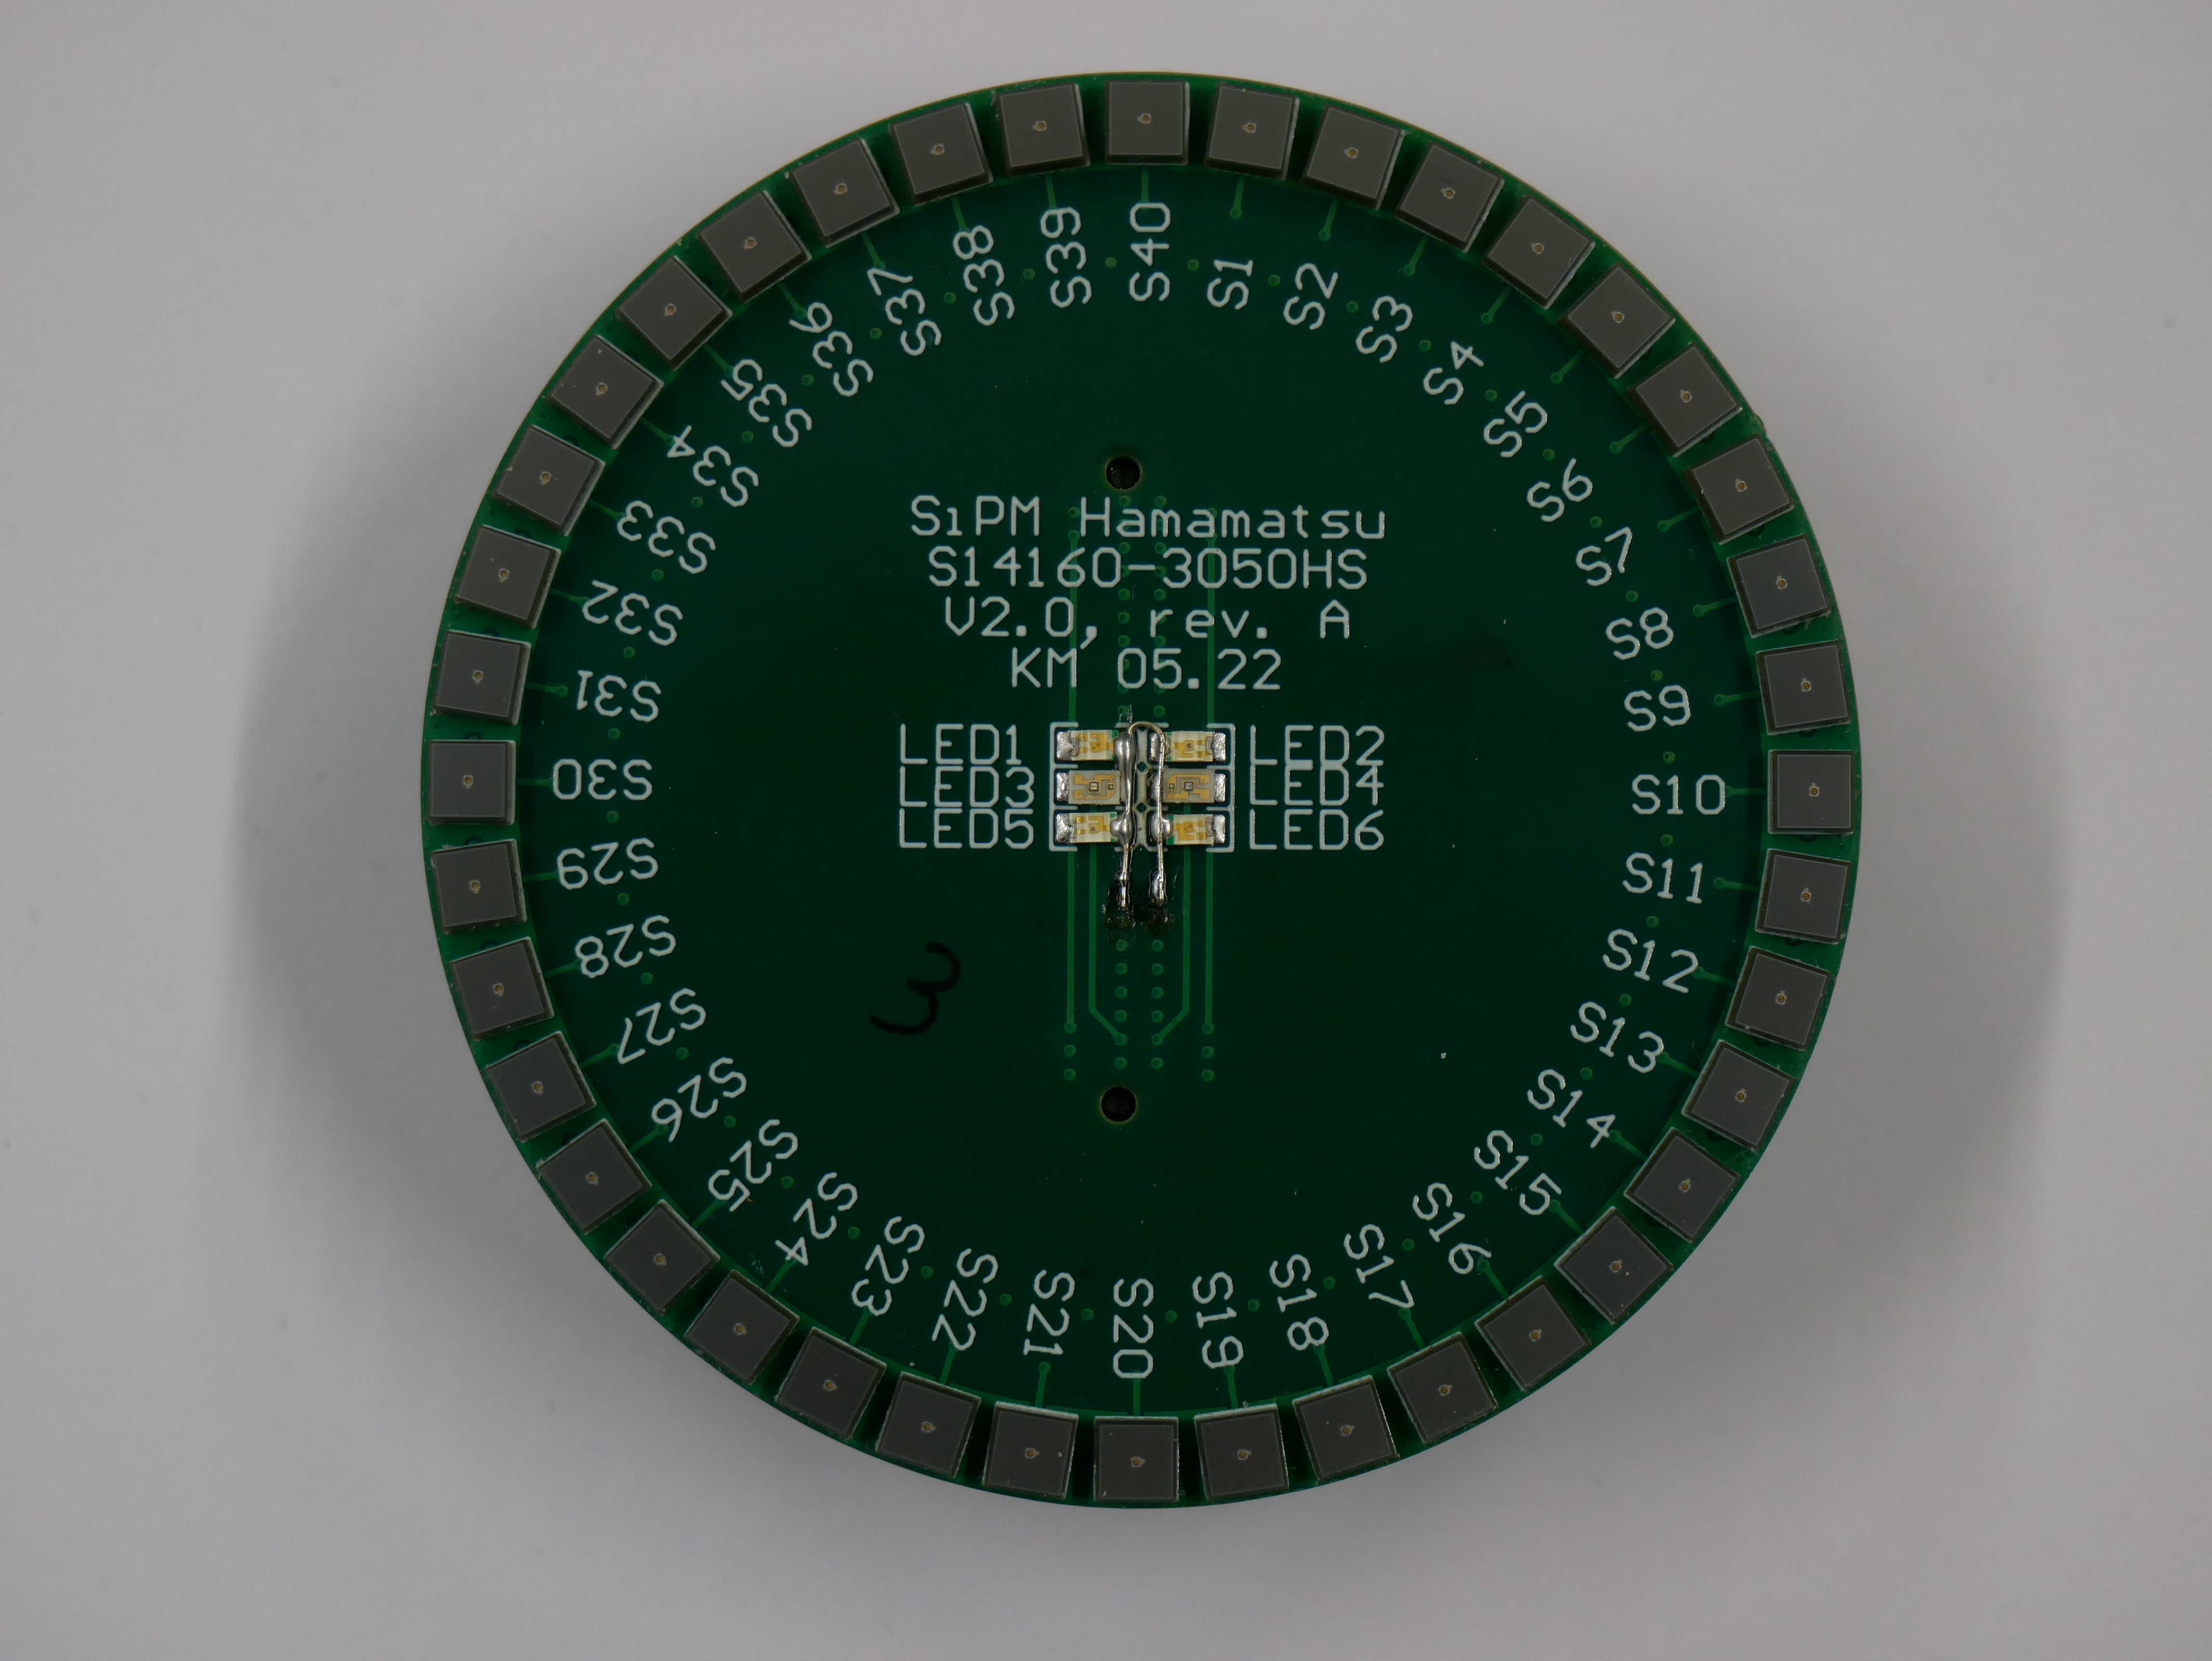
\includegraphics[width=1.\textwidth]{pictures/sipm_ham_pcb}
	\caption[\ac{pcb} with Hamamatsu \acp{sipm}]{One of the \acp{pcb} with Hamamatsu \acp{sipm} used for this work.}
	\label{fig:sipm_pcb}
\end{figure}

\section{dark box stuff}


\section{Gandalf Stuff}

For the operation of the One Cell Prototype sixteen channels need to be digitized, eight of each of the two \acp{wom}.
Therefore two \acp{gandalf} are required.
In order to save place and simplify the setup, the \acp{gandalf} are not operated in a VME crate but are each in a \ac{gandalf} portable.
It is a mobile case made exactly for such puroses where a whole crate is unconvinient.
A picture of a \ac{gandalf} portable is shown in \autoref{fig:gandalf_portable}.
Due to the usage of two \acp{gandalf} an external clock is required to ensure a syncronized sampling frequency and clock for time stamps.
As an external clock a copper GIMLI was chosen and used with a GIMLI testboard, shown in \autoref{fig:gimli_testboard}.
It has two slots for GMILIs, for each on data and one clock output and a power connector to supply it with \SI{5}{\volt}.
For the purpose of an external clock, only one of these slots and the corresponding clock output is used.
Via LEMO cables, the clock signal form the boards clock output pins is connected to the clock inputs of the \acp{gandalf}.


